\documentclass[11pt]{ctexart}

\usepackage[margin=2cm,a4paper]{geometry}
\usepackage{minted}
\usepackage[breaklinks]{hyperref}
\usepackage{amsfonts}
\usepackage{amsmath}
\usepackage{mathtools}
% \usepackage{sectsty}
\usepackage{listings}
\usepackage{hyperref}
\usepackage{graphicx}

\catcode`。=\active
\def。{.}
\setmainfont{Caladea}

\hypersetup{
    colorlinks=false,
    pdfborder={0 0 0},
}

\DeclareMathOperator{\Tr}{Tr}
\newcommand{\defn}[2]{\textbf{#1}(#2)}
\newcommand{\tr}{\mathrm{tr}}
\newcommand*{\vertbar}{\rule[-1ex]{0.5pt}{2.5ex}}
\newcommand*{\horzbar}{\rule[.5ex]{2.5ex}{0.5pt}}
\newcommand{\E}{\mathbb{E}}

\makeatletter
\renewcommand*\env@matrix[1][*\c@MaxMatrixCols c]{%
  \hskip -\arraycolsep
  \let\@ifnextchar\new@ifnextchar
  \array{#1}}
\makeatother


% rmfamily:宋体
% textbf:加黑宋体
% textsf:黑体
% textit:开题
% texttt:仿宋

\title{CS229 课程讲义\footnote{授于 Stanford Fall 2009,课程链接\ \url{http://cs229.stanford.edu}}}
	\author{吴恩达\footnote{Andrew Ng}}
	\date{}

\begin{document}

\maketitle
\tableofcontents

\clearpage
\section*{监督学习\ Supervised Learning}

我们先来聊几个使用监督学习来解决问题的实例。假如我们有一个数据集,里面的数据是俄勒冈州波特兰市的47套房屋的面积和价格:

\begin{table}[!h]
\centering
\begin{tabular}{c|c}
Living area (feet$^2$) & Price (1000\$s) \\ \hline
2104               & 400          \\
1600               & 330          \\
2400               & 369          \\
1416               & 232          \\
3000               & 540          \\
\vdots             & \vdots
\end{tabular}
\end{table}

我们可以根据这些数据作图:

\begin{figure}[!h]
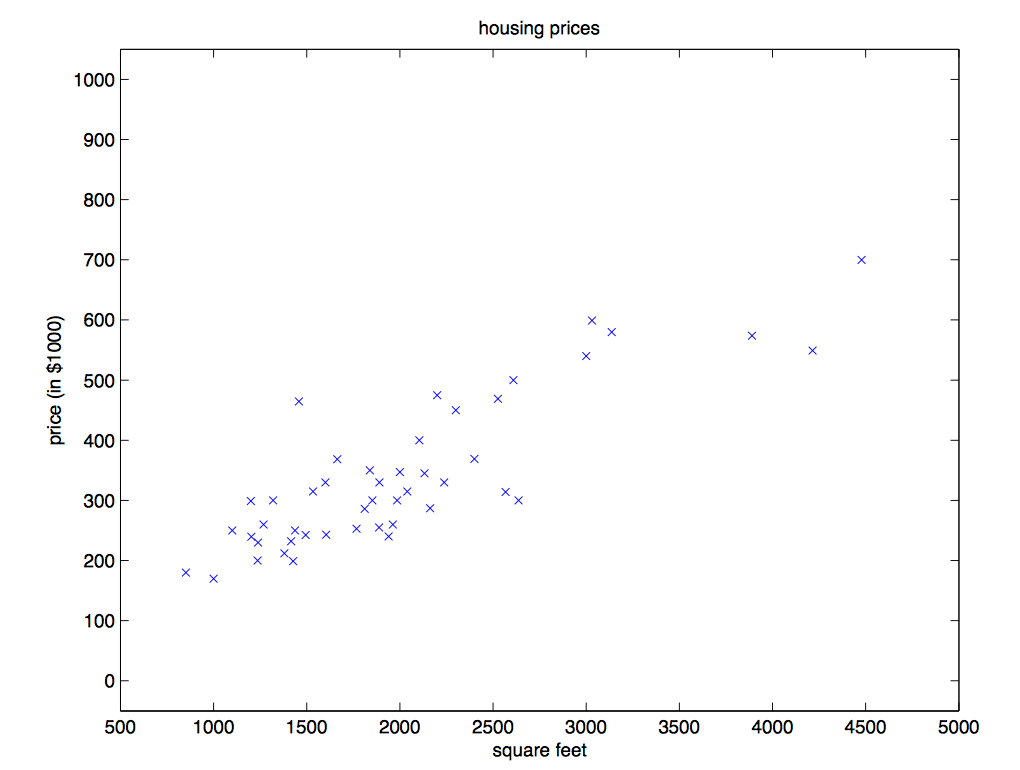
\includegraphics[width=8cm]{house.png}
\centering
\end{figure}

这里要先规范一下符号和含义,这些符号以后还要用到:
我们假设 $x(i)$ 表示“输入的”变量值(在这个例子中就是房屋面积),也可以叫做\defn{输入特征}{input features};
用 $y(i)$ 来表示“输出值”,或称之为我们需要预测的\defn{目标变量}{target variable}(即房屋价格)。
这样的一对 $(x(i),y(i))$ 就称为一组\defn{训练样本}{training example}。
然后我们用来让机器来学习的\defn{数据集}{training set},
就是一个长度为 $m$ 的训练样本的列表,$\{(x(i),y(i)); i=1,\dots,m\}$,也叫做一个训练集。
注意,这里的上标 “$(i)$” 只是作为训练集的索引记号,和数学乘方没有任何关系,千万别误解了。
另外我们会用 $\mathcal{X}$ 来表示输入值的空间,$\mathcal{Y}$ 表示输出值的空间。
在本节的这个例子中,$\mathcal{X}=\mathcal{Y}=\mathbb{R}$。

监督学习的严谨表达方式是这样的:
给定一个训练集,我们的目标是让机器学习函数 $h: \mathcal{X} \mapsto \mathcal{Y}$,使得评估值 $h(x)$ 与真实的 $y$ 值比较接近。
出于历史原因,这个函数 $h$ 被叫做\defn{假设}{hypothesis}。大概如下图(下一页)。

\begin{figure}[!h]
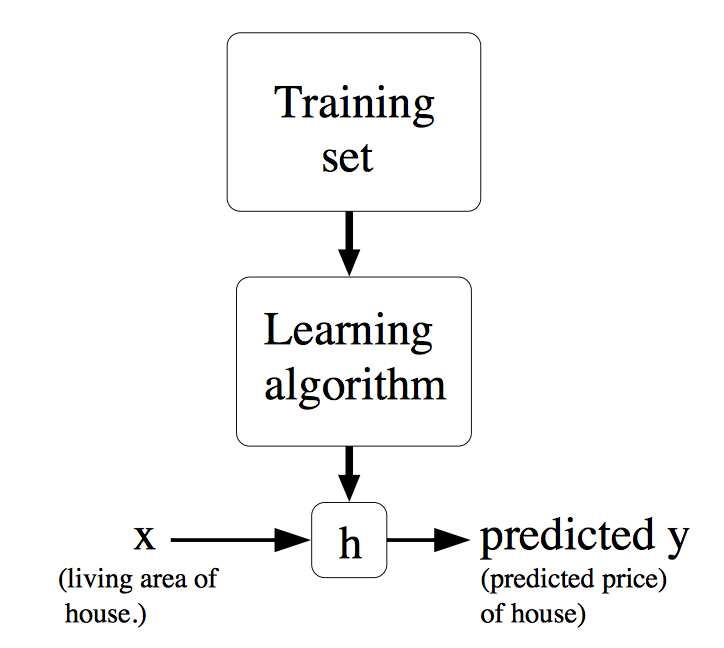
\includegraphics[width=8cm]{training.png}
\centering
\end{figure}

如果我们要预测的目标变量是连续的,比如在我们这个房屋价格-面积的案例中,
这种学习问题就被称为\defn{回归问题}{regression problem}。
如果 $y$ 只能取一小部分的离散的值(比如给定房屋面积,确定这个房子是一个住宅还是公寓),
这样的问题就叫做\defn{分类问题}{classification problem}。




\clearpage
\part{线性回归\ Linear Regression}


为了让这个房屋案例更有意思,我们稍微对数据集进行一下补充,增加上每一个房屋的卧室数目:

\begin{table}[!h]
\centering
\begin{tabular}{c|c|c}
Living area (feet$^2$) & \#bedrooms & Price (1000\$s) \\ \hline
2104               & 3 & 400          \\
1600               & 3 & 330          \\
2400               & 3 & 369          \\
1416               & 2 & 232          \\
3000               & 4 & 540          \\
\vdots             & \vdots & \vdots
\end{tabular}
\end{table}

现在,输入特征 $x$ 就是在 $\mathbb{R}^2$ 范围取值的一个二维向量了。
例如 $x_1^{(i)}$ 是训练集中第 $i$ 个房屋的面积,而 $x_2^{(i)}$ 是训练集中第 i 个房屋的卧室数目。
(通常来说,设计一个学习算法的时候,选择那些输入特征都取决于你,所以如果你不在波特兰收集房屋信息数据,
你也完全可以选择包含其他的特征,例如房屋是否有壁炉,卫生间的数量啊等等。
关于特征筛选的内容会在后面的章节进行更详细的介绍,不过目前来说就暂时先用给定的这两个特征了。)

要进行这个监督学习,我们必须得确定好如何在计算机里面对这个函数/假设 $h$ 进行表示。
现在刚刚开始,就来个简单点的,把 $y$ 假设为一个以 $x$ 为变量的线性函数:
\[
	h_\theta(x) = \theta_0 + \theta_1 x_1 + \theta_2 x_2.
\]
这里的 $\theta_i$ 们是\defn{参数}{parameter}(也可以叫做\defn{权重}{weight}),
是从 $\mathcal{X}$ 到 $\mathcal{Y}$ 的线性函数映射的空间参数。
在不至于引起混淆的情况下,可以把 $h_\theta(x)$ 里面的 $\theta$ 省略掉,简写成 $h(x)$。
另外为了简化公式,设 $x_0 = 1$(即\defn{截距项}{intercept term})。这样简化之后就有了:
\[
	h(x) = \sum_{i=0}^n \theta_i x_i = \theta^T x.
\]
等式的最右边的 $\theta$ 和 $x$ 都是向量,等式中的 $n$ 是输入变量的个数(不包括$x_0$)。

现在,给定了一个训练集了,我们怎么来挑选(学习)参数 $\theta$ 呢?
一个看上去比较合理的方法就是让 $h(x)$ 尽量逼近 $y$,至少对已有的训练样本能适用。
用公式的方式来表示的话,就要定义一个函数,来衡量对于每个不同的 $\theta$ 值,$h(x(i))$ 与对应的 $y(i)$ 的距离。
这样用如下的方式定义了一个\defn{成本函数}{cost function}:
\[
	J(\theta) = {1 \over 2} \sum_{i=1}^m (h_\theta(x^{(i)}) - y^{(i)})^2.
\]
如果之前你接触过线性回归,你会发现这个函数和常规最小二乘法拟合模型中的最小二乘法成本函数非常相似。
不管之前接触过没有,都接着往下进行,以后我们就会发现这是一个更广泛的算法家族中的一个特例。



\section{最小均方算法\ LMS Algorithm}

我们希望选择一个能让 $J(\theta)$ 最小的 $\theta$ 值。怎么做呢,我们先用一个搜索的算法,
从某一个对 $\theta$ 的“初始猜测值”,然后对 $\theta$ 值不断进行调整,来让 $J(\theta)$ 逐渐变小,
最好是直到我们能够达到一个使 $J(\theta)$ 最小的 $\theta$。具体来说,可以考虑使用
\defn{梯度下降法}{gradient descent algorithm},这个方法就是从某一个 $\theta$ 的初始值开始,然后不断更新
\footnote{本文中 “$:=$” 表示赋值操作,是把等号右边的计算结果赋值给左边的变量,注意与等价 “$=$” 区分。}:
\[
	\theta_j := \theta_j - \alpha {\partial \over \partial \theta_j} J(\theta).
\]
(上面的这个更新要同时对应从 $0$ 到 $n$ 的所有 $j$ 值进行。)这里的 $\alpha$ 也称为学习速率。
这个算法是很自然的,逐步重复朝向 $J$ 降低最快的方向移动。要实现这个算法,需要解决等号右边的导数项。
首先来解决只有一组训练样本 $(x, y)$ 的情况,这样就可以忽略掉等号右边对 $J$ 的求和项目了,于是有:
\begin{align*}
	{\partial \over \partial \theta_j} J(\theta)
    	&= {\partial \over \partial \theta_j} {1 \over 2} (h_\theta(x) - y)^2 \\
        &= 2 \cdot {1 \over 2} (h_\theta(x) - y) \cdot {\partial \over \partial \theta_j} (h_\theta(x) - y) \\
        &= (h_\theta(x) - y) \cdot {\partial \over \partial \theta_j} \left( \sum_{i=0}^n \theta_i x_i - y \right) \\
        &= (h_\theta(x) - y) x_j
\end{align*}
对于单个训练样本,更新规则如下所示:
\[
	\theta_j := \theta_j + \alpha(y^{(i)} - h_\theta(x^{(i)}))x_j^{(i)}.
\]

这个也叫做 \defn{最小均方}{LMS,least mean squares} 更新规则,也被称为 Widrow-Hoff 学习规则。
这个规则有几个看上去就很自然直观的特性。例如,更新的大小与\defn{误差项}{error term} $(y(i) − h_\theta(x(i)))$ 成正比;
另外,当我们遇到训练样本的预测值与 $y(i)$ 的真实值非常接近的情况下,就会发现基本没必要再对参数进行修改了;
与此相反的情况是,如果我们的预测值 $h_\theta(x(i))$ 与 $y(i)$ 的真实值有很大的误差(比如距离特别远),那就需要对参数进行更大地调整。

我们推导出了针只有一个训练样本的 LMS 规则。当一个训练集有超过一个训练样本的时候,有两种对这个规则的修改方法。第一种就是下面这个算法:

重复直到收敛 \{
	$\theta_j := \theta_j + \alpha \sum_{i=1}^m (y^{(i)} - h_\theta(x^{(i)}))x_j^{(i)}$
\}

读者很容易能证明,在上面这个更新规则中求和项的值就是 $\partial J(\theta) / \partial \theta_j$ (对 $J$ 的原始定义)。
所以这个更新规则实际上就是对原始的成本函数 $J$ 进行简单的梯度下降。
这一方法在每一个步长内检查所有整个训练集中的所有样本,也叫做\defn{批量梯度下降法}{batch gradient descent}。
注意,因为梯度下降法容易被局部最小值影响,而我们要解决的这个线性回归的优化问题只能有一个全局的而不是局部的最优解;
因此,梯度下降法应该总是收敛到全局最小值(假设学习速率 $\alpha$ 不设置的过大)。
事实上,$J$ 是一个凸的二次函数。下面是一个样例,其中对一个二次函数使用了梯度下降法来找到最小值。

上图的椭圆就是一个二次函数的轮廓图。图中还有梯度下降法生成的规矩,初始点位置在 $(48,30)$。
图中的画的 $x$(用直线连接起来了)标记了梯度下降法所经过的 $\theta$ 的可用值。

对之前的房屋数据集进行批量梯度下降来拟合 $\theta$,把房屋价格当作房屋面积的函数来进行预测,
我们得到的结果是 $\theta_0 = 71.27$, $\theta_1 = 0.1345$。
如果把 $h_\theta(x)$ 作为一个定义域在 $x$ 上的函数来投影,同时也投上训练集中的已有数据点,会得到下图3。
\begin{figure}[!h]
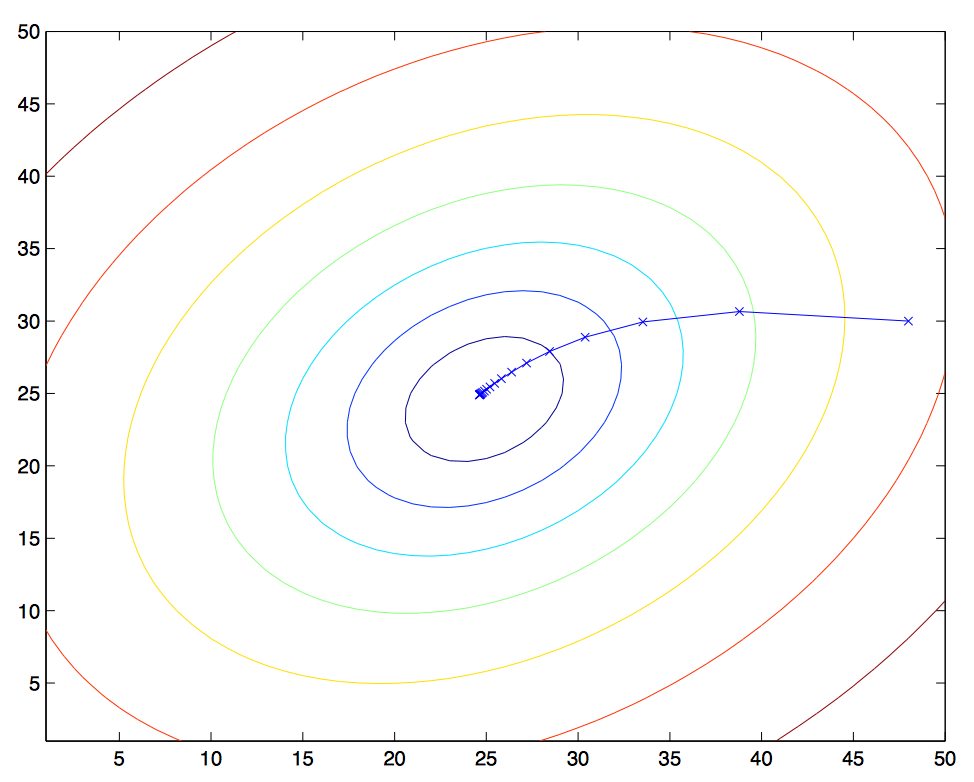
\includegraphics[width=8cm]{1.png}
\centering
\end{figure}

如果在数据集中添加上卧室数目作为输入特征,那么得到的结果就是
$\theta_0 = 89.60$,$\theta_1 = 0.1392$,$\theta_2 = −8.738$。

这个结果就是用批量梯度下降法来获得的。此外还有另外一种方法能够替代批量梯度下降法,这种方法效果也不错。如下所示:
\begin{figure}[!h]
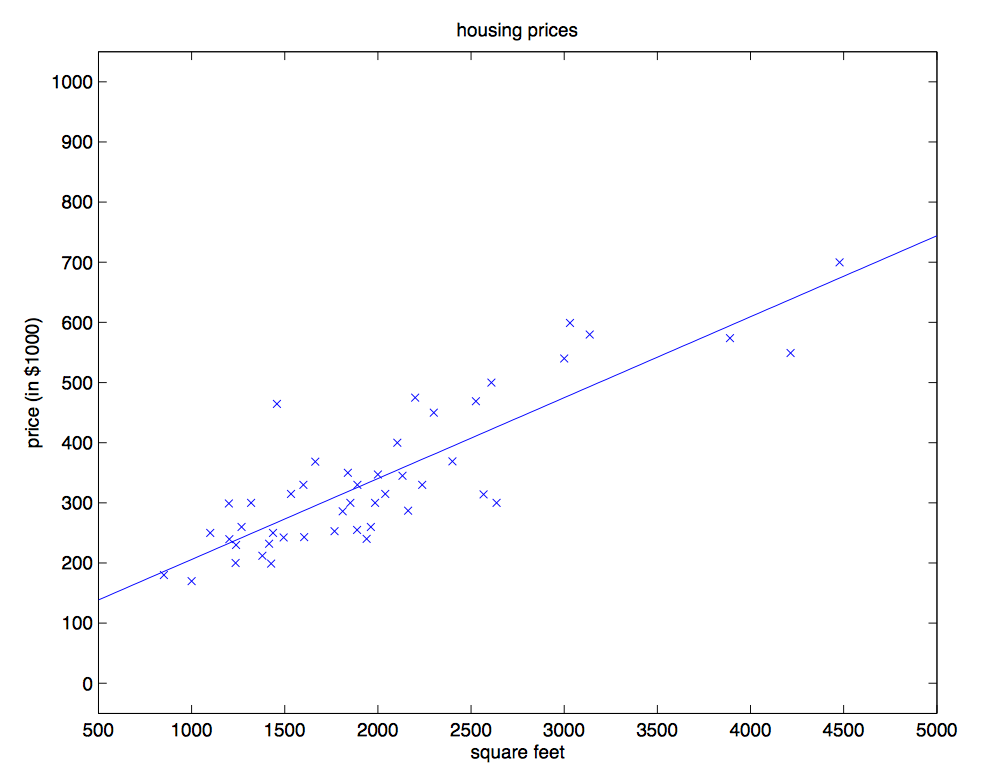
\includegraphics[width=8cm]{2.png}
\centering
\end{figure}

在这个算法里,我们对整个训练集进行了循环遍历,每次遇到一个训练样本,根据每个单一训练样本的误差梯度来对参数进行更新。
这个算法叫做\defn{随机梯度下降法}{stochastic gradient descent},或者叫\defn{增量梯度下降法}{incremental gradient descent}。
批量梯度下降法要在运行第一步之前先对整个训练集进行扫描遍历,当训练集的规模 $m$ 变得很大的时候,因此引起的性能开销就很不划算了;
随机梯度下降法就没有这个问题,而是可以立即开始,对查询到的每个样本都进行运算。
通常情况下,随机梯度下降法查找到足够接近最低值的 $\theta$ 的速度要比批量梯度下降法更快一些。
(注意,也有可能会一直无法\defn{收敛}{converge}到最小值,这时候 $\theta$ 会一直在 $J(\theta)$ 最小值附近震荡;
不过通常情况下在最小值附近的这些值大多数其实也足够逼近了,足以满足精度要求,所以也可以用
\footnote{此外很常见的情况通常是我们事先对数据集已经有了描述,并且有了一个确定的学习速率 $\alpha$,然后来运行随机梯度下降,
同时逐渐让学习速率 $\alpha$ 随着算法的运行而逐渐趋于 $0$,这样也能保证我们最后得到的参数会收敛到最小值,
而不是在最小值范围进行震荡。})由于以上种种原因,通常更推荐使用的都是随机梯度下降法,而不是批量梯度下降法,尤其是在训练用的数据集规模大的时候。 





\section{法线方程\ The Normal Equations}

上文中的梯度下降法是一种找出 $J$ 最小值的办法。我们再聊一聊另一种实现方法,这种方法寻找起来简单明了,
而且不需要使用迭代算法:我们直接利用找对应导数为 $0$ 位置的 $\theta_j$,这样就能找到 $J$ 的最小值了。
我们想实现这个目的,还不想写一大堆代数公式或者好几页的矩阵积分,所以就要介绍一些做矩阵积分的记号。

\subsection{矩阵导数\ Matrix Derivatives}

对于一个从 $m \times n$ 大小的矩阵映射到实数域的函数 $f: \mathbb{R}^{m \times n} \mapsto \mathbb{R}$,
定义 $f$ 对 $A$ 的导数为:
\[
	\nabla_A f(A) = \begin{bmatrix}
    	{\partial f \over \partial A_{11}} & \cdots & {\partial f \over \partial A_{1n}} \\
        \vdots & \ddots & \vdots \\
        {\partial f \over \partial A_{m1}} & \cdots & {\partial f \over \partial A_{mn}}
    \end{bmatrix}
\]
因此,这个梯度 $\nabla_A f(A)$ 本身也是一个 $m \times n$ 的矩阵,其中第 $(i,j)$ 个元素是 $\partial f / \partial A_{ij}$。
例如,令矩阵 $A = \begin{bmatrix} A_{11} & A_{12} \\ A_{21} & A_{22} \end{bmatrix}$,
定义函数 $f: \mathbb{R}^{2 \times 2} \mapsto \mathbb{R}$ 为 $f(A) = {3 \over 2} A_{11} + 5A_{12}^2 + A_{21}A_{22}$,
有 $\nabla_A f(A) = \begin{bmatrix} 3/2 & 10 A_{12} \\ A_{22} & A_{21} \end{bmatrix}$。

此外,这里还要介绍求\defn{迹}{trace}运算,记作 $\tr$。对于一个 $n \times n$ 方阵 $A$,$A$ 的迹定义为其对角线之和:
\[
	\tr A = \sum_{i=1}^n A_{ii}.
\]
假如 $a$ 是一个实数,实际上就可以看做是一个 $1 \times 1$ 的矩阵,那么就有 $a$ 的迹 $\tr a = a$。
(如果你之前没有见到过这种算子写法,就可以把 $A$ 的迹看成是 $\tr(A)$,
或者理解成为一个对矩阵 $A$ 进行操作的 \texttt{trace} 函数。不过通常情况都是写成不带括号的形式更多一些。) 

如果有两个矩阵 $A$ 和 $B$,能够满足 $AB$ 为方阵,求迹运算就有一个特殊的性质:$\tr AB = \tr BA$。
(自己想办法证明!)在此基础上进行推论,就能得到类似下面这样的等式关系:
\begin{gather*}
	\tr ABC = \tr CAB = \tr BCA, \\
    \tr ABCD = \tr DABC = \tr CDAB = \tr BCDA
\end{gather*}
下面这些和求迹运算相关的等量关系也很容易证明。其中 $A$ 和 $B$ 都是方阵,$a$ 是一个实数:
\begin{align*}
	\tr A &= \tr A^T \\
    \tr(A+B) &= \tr A + \tr B \\
    \tr aA &= a \tr A
\end{align*}

接下来在不进行证明的情况下提出一些矩阵导数(其中的一些直到本节末尾才用得上)。
另外要注意最后一个等式中 $A$ 必须是\defn{非奇异方阵}{non-singular square matrices},而 $|A|$ 表示的是矩阵 $A$ 的行列式:
\begin{align}
	\nabla_A \tr AB &= B^T \\
    \nabla_{A^T} f(A) &= (\nabla_A f(A))^T \\
    \nabla_A \tr ABA^TC &= CAB + C^TAB^T \\
    \nabla_A |A| &= |A|(A^{-1})^T
\end{align}

为了让我们的矩阵运算记号更加具体,在此详细解释一下这些等式中的第一个。
假定我们有一个确定的矩阵 $B \in \mathbb{R}^{n \times m}$,
那么接下来就可以定义一个函数 $f: \mathbb{R}^{m \times n} \mapsto \mathbb{R}$ 对应这里的 $f(A) = \tr AB$。
注意,这个矩阵是有意义的,因为如果 $A \in \mathbb{R}^{m \times n}$,那么 $AB$ 就是一个方阵,是方阵就可以求迹;
因此,实际上 $f$ 映射的是从 $\mathbb{R}^{m\times n}$ 到实数域 $\mathbb{R}$。
这样接下来就可以使用矩阵导数来找到 $\nabla_A f(A)$ ,这个导函数本身也是一个 $m \times n$ 的矩阵。
上面的等式 $(1)$ 表明了这个导数矩阵的第 $(i, j)$ 个元素等同于 $B^T$ ($B$ 的转置)的第 $(i, j)$ 个元素,或者更直接表示成 $B_{ji}$。 
等式 $(1-3)$ 都很简单,证明就都留给读者做练习了。等式 $(4)$ 需要用逆矩阵的伴随矩阵来推导出
\footnote{假如我们定义一个矩阵 $A′$,它的第 $(i, j)$ 个元素是 $(−1)^{i+j}$ 与矩阵 $A$ 去除第 $i$ 行和第 $j$ 列后的行列式的乘积,
则可以证明有 $A^{−1} = (A′)^T / |A|$。(你可以验证,比如在 $A$ 是一个 $2 \times 2$ 矩阵的情况下看看 $A^{-1}$ 是什么样的,
然后以此类推。如果你想看看对于这一类结果的证明,可以参考一本中级或者高级的线性代数教材,
比如 Charles Curtis, 1991, \textit{Linear Algebra}, Springer)这也就意味着 $A′ = |A|(A^{−1})^T$ 。
此外,一个矩阵 $A$ 的行列式也可以写成 $|A| = \sum_j A_{ij}A′$ 。因为 $(A′)_{ij}$ 不依赖 $A_{ij}$
(通过定义也能看出来),这也就意味着 $(\partial / \partial A_{ij})|A| = A′_{ij}$,综合起来也就得到上面的这个结果了。}。

\subsection{最小二乘法回顾\ Least Squares Revisited}

通过刚才的内容,我们大概掌握了矩阵导数这一工具,接下来就继续用\defn{逼近模型}{closed-form}
来找到能让 $J(\theta)$ 最小的 $\theta$ 值。首先我们把 $J$ 用矩阵-向量的记号来重新表述。
给定一个训练集,定义\defn{设计矩阵}{design matrix} $X$ 为一个 $m \times n$ 矩阵
(实际上,如果考虑到截距项,也就是 $\theta_0$ 那一项,就应该是 $m \times (n+1)$ 矩阵),
这个矩阵里面包含了训练样本的输入值作为每一行
\[
	X = \left[\begin{array}{ccc}
    \horzbar & (x^{(1)})^T & \horzbar \\
    \horzbar & (x^{(2)})^T & \horzbar \\
    & \vdots & \\
    \horzbar & (x^{(m)})^T & \horzbar
    \end{array}\right].
\]
令 $\vec{y}$ 为一个包含了训练集中所有目标值的 $m$ 维向量
\[
	\vec{y} = \left[\begin{array}{c}
    y^{(1)} \\
    y^{(2)} \\
    \vdots \\
    y^{(3)}
    \end{array}\right].
\]
现在,因为 $h_\theta(x^{(i)}) = (x^{(i)})^T \theta$,可以证明
\[
	X\theta - \vec{y}
    = \begin{bmatrix} (x^{(1)})^T\theta \\ \vdots \\ (x^{(m)})^T\theta \end{bmatrix}
    - \begin{bmatrix} y^{(1)} \\ \vdots \\ y^{(1)} \end{bmatrix}
    = \begin{bmatrix} h_\theta(x^{(1)})-y^{(1)} \\ \vdots \\ h_\theta(x^{(m)})-y^{(m)} \end{bmatrix}.
\]
对于向量 $z$ ,则有 $z^T z = \sum_i z_i^2$,因此利用这个性质,可以推出
\[
	{1\over2}(X\theta - \vec{y})^T(X\theta - \vec{y})
    = {1\over2} \sum_{i=1}^m (h_\theta(x^{(i)})-y^{(i)})^2
    = J(\theta).
\]
最后,要让 $J$ 的值最小,就要找到导数为 $0$ 的点。结合等式 $(2)$ 和等式 $(3)$,就能得到下面这个等式 $(5)$:
\begin{equation}
	\nabla_{A^T} \tr ABA^TC = B^TA^TC^T + BA^TC.
\end{equation}
因此就有:
\begin{align*}
	\nabla_\theta J(\theta)
    	&= \nabla_\theta {1\over2}(X\theta - \vec{y})^T(X\theta - \vec{y}) \\
        &= {1\over2} \nabla_\theta (\theta^T X^T X \theta - \theta^T X^T \vec{y} - \vec{y}^T X \theta + \vec{y}^T \vec{y}) \\
        &= {1\over2} \nabla_\theta \tr (\theta^T X^T X \theta - \theta^T X^T \vec{y} - \vec{y}^T X \theta + \vec{y}^T \vec{y}) \\
        &= {1\over2} \nabla_\theta (\tr \theta^T X^T X - 2 \tr \vec{y}^T X \theta) \\
		&= {1\over2} (X^T X \theta + X^T X \theta - 2 X^T \vec{y}) \\
        &= X^T X \theta - X^T \vec{y}.
\end{align*}
在第三步,我们用到了一个定理,也就是一个实数的迹就是这个实数本身;
第四步用到了 $\tr A = \tr A^T$ 这个定理;
第五步用到了等式 $(5)$,其中 $A^T = \theta$, $B=B^T=X^TX$, $C=I$,还用到了等式 (1)。
要让 $J$ 取得最小值,就令其导数为 $0$,然后就得到了下面的\defn{法线方程}{normal equations}:
\[
	X^T X \theta - X^T \vec{y}.
\]
所以让 $J(\theta)$ 取值最小的 $\theta$ 就是
\[
	\theta = (X^TX)^{-1}X^T\vec{y}.
\]





\section{概率观点解释\ Probabilistic Interpretation}

在面对回归问题的时候,可能有这样一些疑问,就是为什么选择线性回归,尤其是为什么而是最小二乘法成本函数 $J$?
在本节里,我们会给出一系列的概率基本假设,基于这些假设,就可以推出最小二乘法回归是一种非常自然的算法。

首先假设目标变量和输入值存在下面这种等量关系: 
\[
	y^{(i)} = \theta^T x^{(i)} + \epsilon^{(i)}.
\]
其中 $\epsilon^{(i)}$ 是误差项,用于存放由于建模所忽略的变量导致的效果
(比如可能某些特征对于房价的影响很明显,但我们做回归的时候忽略掉了)或者随机的\defn{噪音信息}{random noise}。
进一步假设 $\epsilon^{(i)}$ 是\defn{独立同分布的}{i.i.d., independently and identically distributed},
服从\defn{高斯分布}{Gaussian distribution},也叫\defn{正态分布}{Normal distribution},
其平均值为 $0$,方差为 $\sigma^2$。这样就可以把这个假设写成 $\epsilon^{(i)} \sim \mathcal{N}(0,\sigma^2)$。
所以 $\epsilon^{(i)}$ 的密度函数就是:
\[
	p(\epsilon^{(i)}) 
    = {1 \over \sqrt{2\pi} \sigma} \exp\left\{ -{(\epsilon^{(i)})^2 \over 2 \sigma^2} \right\}.
\]
即
\[
	p(y^{(i)} | x^{(i)}; \theta) 
    = {1 \over \sqrt{2\pi} \sigma} \exp\left\{ -{(y^{(i)}-\theta^T x^{i})^2 \over 2 \sigma^2} \right\}.
\]
这里的记号 “$p(y(i)|x(i); \theta)$” 表示的是这是一个对于给定 $x(i)$ 的 $y(i)$ 的分布,用 $\theta$ 进行了参数化。
注意这里不能用 $\theta$ 来当做条件,因为它并不是一个随机变量。
这个 $y(i)$ 的分布还可以写成 $y(i) | x(i); \theta \sim \mathcal{N}(\theta^T x(i), \sigma^2)$。

给定一个 $X$ 为设计矩阵,包含了全部 $x(i)$,然后再给定 $\theta$,那么 $y(i)$ 的分布是什么?
数据的概率以 $p(\vec{y}|X;\theta)$ 的形式给出。在 $\theta$ 取某个固定值的情况下,
这个等式通常可以看做是一个 $\vec{y}$ 的函数(也可以看成是 $X$ 的函数)。
当我们要把它当做 $\theta$ 的函数的时候,就称它为\defn{似然函数}{likelihood function}:
\[
	L(\theta) = L(\theta; X, \vec{y}) = p(\vec{y}|X; \theta).
\]
结合之前对 $\epsilon^{(i)}$ 的独立性假设(这里对 $y(i)$ 以及给定的 $x(i)$ 也都做同样假设),就可以把上面这个等式改写成下面的形式:
\[
	L(\theta)
    	= \prod_{i=1}^m p(y^{(i)} | x^{(i)}; \theta)
        = \prod_{i=1}^m {1 \over \sqrt{2\pi} \sigma} \exp\left\{ -{(y^{(i)}-\theta^T x^{i})^2 \over 2 \sigma^2} \right\}.
\]

现在,给定了 $y(i)$ 和 $x(i)$ 之间关系的概率模型了,用什么方法来选择我们对参数 $\theta$ 的最佳猜测呢?
\defn{最大似然法}{maximum likelihood}告诉我们要选择能让数据的似然函数尽可能大的 $\theta$。
也就是说,我们要找的 $\theta$ 能够让函数 $L(\theta)$ 取到最大值。

除了找到 $L(\theta)$ 最大值,我们还以对任何严格递增的 $L(\theta)$ 的函数求最大值。
如果我们不直接使用 $L(\theta)$,而是使用对数函数,来找\defn{对数似然}{log likelihood} $\ell(\theta)$ 的最大值,
那这样对于求导来说就简单了一些: 
\begin{align*}
	\ell(\theta)
    	&= \log L(\theta) \\
        &= \log \prod_{i=1}^m {1 \over \sqrt{2\pi} \sigma}
           \exp\left\{ -{(y^{(i)}-\theta^T x^{i})^2 \over 2 \sigma^2} \right\} \\
        &= \sum_{i=1}^m \log {1 \over \sqrt{2\pi} \sigma}
           \exp\left\{ -{(y^{(i)}-\theta^T x^{i})^2 \over 2 \sigma^2} \right\} \\
        &= m \log {1 \over \sqrt{2\pi} \sigma} - {1 \over \sigma^2} \cdot {1 \over 2}
           \sum_{i=1}^m (y^{(i)}-\theta^T x^{i})^2.
\end{align*}
因此,对 $\ell(\theta)$ 的最大值也就意味着下面这个子式取到最小值:
\[
	{1 \over 2} \sum_{i=1}^m (y^{(i)}-\theta^T x^{i})^2.
\]
到这里我们能发现这个子式实际上就是 $J(\theta)$,也就是最原始的最小二乘成本函数。

总结一下:在对数据进行概率假设的基础上,最小二乘回归得到的 $\theta$ 和最大似然法估计的 $\theta$ 是一致的。
所以这是一系列的假设,其前提是认为最小二乘回归能够被判定为一种非常自然的方法,这种方法正好就进行了最大似然估计。
(要注意,对于验证最小二乘法是否为一个良好并且合理的过程来说,这些概率假设并不是必须的,
此外可能有其他的自然假设(确实有)能够用来评判最小二乘方法。)

另外还要注意,在刚才的讨论中,我们最终对 $\theta$ 的选择并不依赖 $\sigma^2$,
而且也确实在不知道 $\sigma^2$ 的情况下就已经找到了结果。稍后我们还要对这个情况加以利用,到时候我们会讨论指数族以及广义线性模型。






\section{局部加权线性回归\ Locally Weighted Linear Regression}

假如问题还是根据从实数域内取值的 $x \in \mathbb{R}$ 来预测 $y$ 。
左下角的图显示了使用 $y = \theta_0 + \theta_1x$ 来对一个数据集进行拟合。
我们明显能看出来这个数据的趋势并不是一条严格的直线,所以用直线进行的拟合不是好的方法。

\begin{figure}[!h]
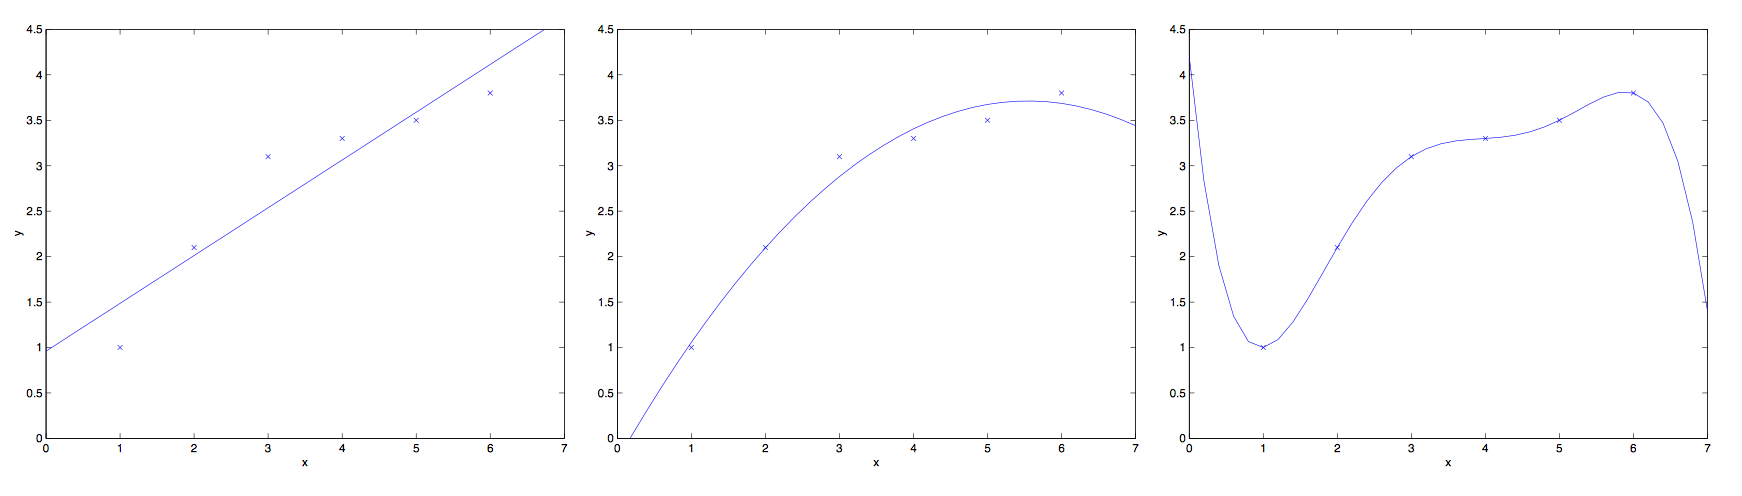
\includegraphics[width=\textwidth]{3.png}
\centering
\end{figure}

那么这次不用直线,而增加一个二次项,用 $y = \theta_0 + \theta_1x + \theta_2x^2$ 来拟合。
(看中间的图)很明显,我们对特征补充得越多,效果就越好。
不过,增加太多特征也会造成危险的:最右边的图就是使用了五次多项式 $y = \sum_{j=0}^5 \theta_j x^j$ 来进行拟合。
看图就能发现,虽然这个拟合曲线完美地通过了所有当前数据集中的数据,但我们明显不能认为这个曲线是一个合适的预测工具,
比如针对不同的居住面积 $x$ 来预测房屋价格 $y$。先不说这些特殊名词的正式定义,
简单来说,最左边的图像就是一个\defn{欠拟合}{under fitting}的例子,比如明显能看出拟合的模型漏掉了数据集中的结构信息;
而最右边的图像就是一个\defn{过拟合}{over fitting}的例子。
(在本课程的后续部分中,当我们讨论到关于学习理论的时候,会给出这些概念的标准定义,也会给出拟合程度对于一个猜测的好坏检验的意义。)

正如前文谈到的,也正如上面这个例子展示的,一个学习算法要保证能良好运行,特征的选择是非常重要的。
(等到我们讲模型选择的时候,还会看到一些算法能够自动来选择一个良好的特征集。)
在本节,我们就简要地讲一下\defn{局部加权线性回归}{LWR, locally weighted linear regression},
这个方法是假设有足够多的训练数据,对不太重要的特征进行一些筛选。
这部分内容会比较简略,因为在作业中会要求学生自己去探索一下 LWR 算法的各种性质。

在原始的线性回归算法中,要对一个查询点 $x$ 进行预测,比如要衡量 $h(x)$,要经过下面的步骤:
\begin{enumerate}
\item 使用参数 $\theta$ 进行拟合,让数据集中的值与拟合算出的值的差值平方 $(y(i) − \theta^T x(i))^2$ 最小;
\item 输出 $\theta^T x$。
\end{enumerate}

相应地,在 LWR 方法中,步骤如下: 
\begin{enumerate}
\item 使用参数 $\theta$ 进行拟合,让加权距离 $\sum_i w^{(i)}(y^{(i)} − \theta^T x(i))^2$ 最小;
\item 输出 $\theta^T x$。
\end{enumerate}

上面式子中的 $w^{(i)}$ 是非负的权值。直观点说就是,如果对应某个 $i$ 的权值 $w^{(i)}$ 特别大,
那么在选择拟合参数 $\theta$ 的时候,就要尽量让这一点的 $(y^{(i)} - \theta^T x(i))^2$  最小。
而如果权值 $w^{(i)}$ 特别小,那么这一点对应的 $(y^{(i)} - \theta^T x(i))^2$ 就基本在拟合过程中忽略掉了。

对于权值的选取可以使用下面这个比较常见的公式
\footnote{如果 $x$ 是有值的向量,那就要对上面的式子进行泛化,得到的是
$w^{(i)} = \exp (−(x^{(i)} - x)^T (x^{(i)} - x)/(2 \tau^2))$,
或者 $w^{(i)} = \exp (−(x^{(i)} - x)^T \Sigma^{-1} (x^{(i)} - x)/ 2)$,这就看是选择用 $\tau$ 还是 $\Sigma$。
}
\[
	w^{(i)} = \exp \left\{ - {(x^{(i)} - x)^2 \over 2\tau^2} \right\}.
\]

要注意的是,权值是依赖每个特定的点 $x$ 的,而这些点正是我们要去进行预测评估的点。
此外,如果 $|x^{(i)} − x|$ 非常小,那么权值 $w^{(i)}$ 就接近 $1$;
反之如果 $|x^{(i)} − x|$ 非常大,那么权值 $w^{(i)}$ 就变小。
所以可以看出,$\theta$ 的选择过程中,查询点 $x$ 附近的训练样本有更高得多的权值。
(还要注意,当权值的方程的形式跟高斯分布的密度函数比较接近的时候,权值和高斯分布并没有什么直接联系,
尤其是当权值不是随机值,且呈现正态分布或者其他形式分布的时候。)

随着点 $x^{(i)}$ 到查询点 $x$ 的距离降低,训练样本的权值的也在降低,
参数 $\tau$ 控制了这个降低的速度;$\tau$ 也叫做\defn{带宽参数}{bandwidth parameter},
这个也是在你的作业中需要来体验和尝试的一个参数。

局部加权线性回归是我们接触的第一个\defn{非参数算法}{non-parametric algorithm}。
而更早之前我们看到的无权重的线性回归算法就是一种\defn{参数算法}{parametric algorithm},
因为有固定的有限个数的参数(也就是 $\theta_i$),这些参数用来拟合数据。我们对 $\theta_i$ 进行了拟合之后,
就把它们存了起来,也就不需要再保留训练数据样本来进行更进一步的预测了。与之相反,如果用局部加权线性回归算法,
我们就必须一直保留着整个训练集。这里的非参数算法中的非参数是说(粗略地):为了呈现出假设 $h$ 随着数据集规模的增长而线性增长,
我们需要以一定顺序保存一些数据的规模。




\clearpage
\part{分类和逻辑回归\ Classification and Logistic Regression}

接下来讲一下分类的问题。分类问题其实和回归问题很像,只不过我们现在要来预测的 $y$ 的值只局限于少数的若干个离散值。
眼下我们首先关注的是二值化分类问题,也就是说我们要判断的 $y$ 只有两个取值,$0$ 或者 $1$。
(我们这里谈到的大部分内容也都可以扩展到多种类的情况。)
例如,假如要建立一个垃圾邮件筛选器,那么就可以用 $x^{(i)}$ 表示一个邮件中的若干特征,
然后如果这个邮件是垃圾邮件,$y$ 就设为 $1$,否则 $y$ 为 $0$。$0$ 也可以被称为\defn{消极类别}{negative class},
而 $1$ 就成为\defn{积极类别}{positive class},有的情况下也分别表示成“$-$”和“$+$”。
对于给定的一个 $x^{(i)}$,对应的 $y^{(i)}$ 也称为训练样本的\defn{标签}{label}。






\section{逻辑回归\ Logistic Regression}

我们当然也可以还按照之前的线性回归的算法来根据给定的 $x$ 来预测 $y$,只要忽略掉 $y$ 是一个散列值就可以了。
然而,这样构建的例子很容易遇到性能问题,这个方法运行效率会非常低,效果很差。
而且从直观上来看,$h_\theta(x)$ 的值如果大于 $1$ 或者小于 $0$ 就都没有意义了,因为已经确定了 $y\in\{0,1\}$,
就是说 $y$ 必然应当是 $0$ 和 $1$ 这两个值当中的一个。
所以我们就改变一下假设函数 $h_\theta(x)$ 的形式,来解决这个问题。比如我们可以选择下面这个函数:
\[
	h_\theta(x) = g(\theta^T x) = {1 \over 1 + e^{\theta^T}x},
\]
其中
\[
	g(z) = {1 \over 1 + e^{-z}}
\]
叫做\defn{逻辑函数}{logistic function},或者也叫\defn{双弯曲S型函数}{sigmoid function}。
下图是 $g(z)$ 的函数图像:

\begin{figure}[!h]
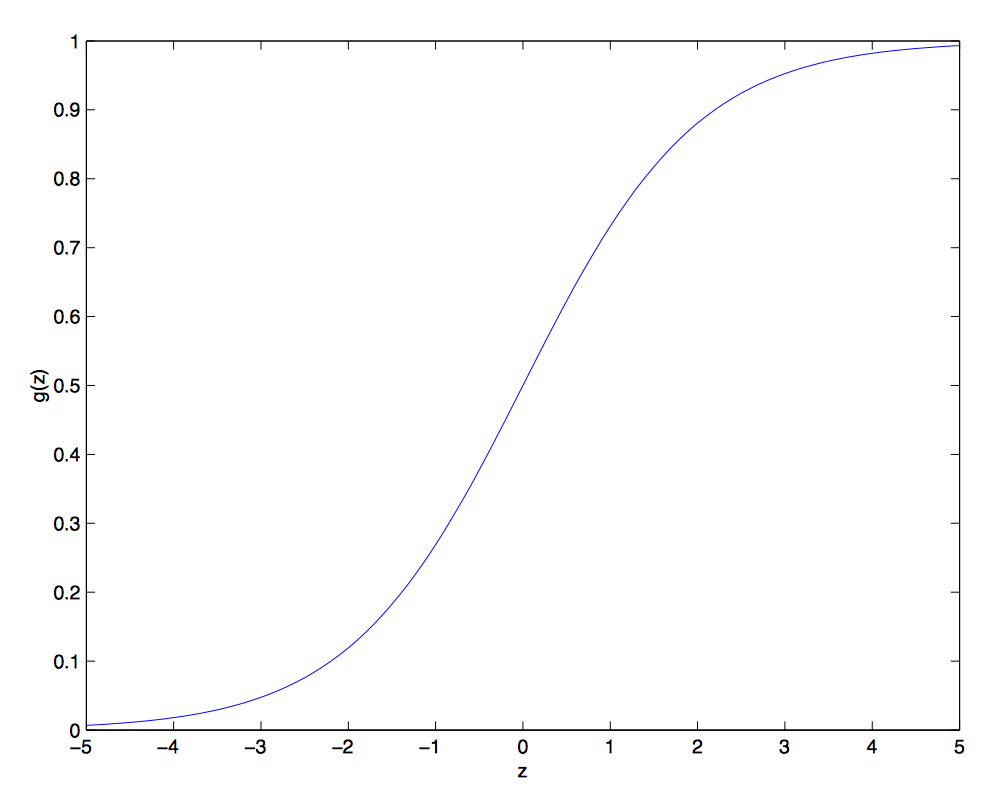
\includegraphics[width=8cm]{4.png}
\centering
\end{figure}

注意,当 $z\rightarrow\infty$ 的时候 $g(z)$ 趋向于 $1$,而当 $z\rightarrow-\infty$ 时 $g(z)$ 趋向于 $0$。
此外,这里的这个 $g(z)$ ,也就是 $h(x)$,是一直在 $0$ 和 $1$ 之间波动的。
然后依然像最开始那样来设置 $x_0 = 1$,这样就有了 $\theta^Tx = \theta_0 + \sum_{j=1}^n \theta_j x_j$。

现在我们就把 $g$ 作为选定的函数了。当然其他的从 $0$ 到 $1$ 之间光滑递增的函数也可以使用,
不过后面我们会了解到选择 $g$ 的一些原因(到时候我们\defn{讲广义线性模型}{GLM, Generalized Linear Model},
那时候还会讲\defn{生成学习算法}{generative learning algorithms}),对这个逻辑函数的选择是很自然的。
在继续深入之前,下面是要讲解的关于这个 S 型函数的导数,也就是 $g′$ 的一些性质:
\begin{align*}
	g'(z)
    	&= {d \over dz} {1 \over 1 + e^{-z}} \\
    	&= {1 \over (1 + e^{-z})^2}(e^{-z}) \\
        &= {1 \over (1 + e^{-z})} \left(1 - {1 \over 1 + e^{-z}}\right) \\
        &= g(z)(1-g(z)).
\end{align*}

那么,给定了逻辑回归模型了,我们怎么去拟合一个合适的 $\theta$ 呢?我们之前已经看到了在一系列假设的前提下,
最小二乘法回归可以通过最大似然估计来推出,那么接下来就给我们的这个分类模型做一系列的统计学假设,
然后用最大似然法来拟合参数吧。

首先假设
\begin{align*}
	P(y=1 | x; \theta) &= h_\theta(x) \\
    P(y=0 | x; \theta) &= 1-h_\theta(x).
\end{align*}
更简洁的写法是
\[
	p(y|x;\theta) = (h_\theta(x))^y (1-h_\theta(x))^{1-y}.
\]
假设 $m$ 个训练样本都是各自独立生成的,那么就可以按如下的方式来写参数的似然函数
\begin{align*}
	L(\theta)
    	&= p(\vec{y} | X; \theta) \\
	    &= \prod_{i=1}^m p(y^{(i)} | x^{(i)}; \theta) \\
        &= \prod_{i=1}^m (h_\theta (x^{(i)}))^{y^{(i)}} (1-h_\theta (x^{(i)}))^{1-y^{(i)}} 
\end{align*}
然后还是跟之前一样,去个对数就更容易计算最大值:
\begin{align*}
	\ell(\theta)
    	&= \log L(\theta) \\
        &= \sum_{i=1}^m y^{(i)} \log h (h^{(i)}) + (1-y^{(i)}) \log(1 - h(x^{(i)}))
\end{align*}

怎么让似然函数最大?就跟之前我们在线性回归的时候用了求导数的方法类似,我们这次就是用\defn{梯度上升法}{gradient ascent}。
还是写成向量的形式,然后进行更新,也就是 $\theta := \theta + \alpha \nabla_\theta \ell(\theta)$。
(注意更新方程中用的是加号而不是减号,因为我们现在是在找一个函数的最大值,而不是找最小值了。)
还是先从只有一组训练样本 $(x,y)$ 来开始,然后求导数来退出随机梯度上升规则:
\begin{align*}
	{\partial \over \partial \theta_j} \ell(\theta)
    	&= \left( y {1 \over g(\theta^T x)} - (1-y) {1 \over 1-g(\theta^T)x}\right) 
           {\partial \over \partial \theta_j} g(\theta^T x) \\
        &= \left( y {1 \over g(\theta^T x)} - (1-y) {1 \over 1-g(\theta^T)x}\right) 
           g(\theta^T x) (1-g(\theta^T x)) {\partial \over \partial \theta_j} \theta^Tx \\
        &= (y (1 - g(\theta^T x)) - (1-y)g(\theta^Tx)) x_j \\
        &= (y - h_\theta(x)) x_j.
\end{align*}
上面的式子里,我们用到了对函数求导的定理 $g'(z) = g(z)(1-g(z))$。然后就得到了随机梯度上升规则:
\[
	\theta_j := \theta_j + \alpha(y^{(i)} - h_\theta(x^{(i)})) x^{(i)}_j.
\]
如果跟之前的 LMS 更新规则相对比,就能发现看上去挺相似的;不过这并不是同一个算法,
因为这里的 $h_\theta(x(i))$ 现在定义成了一个 $\theta^Tx(i)$ 的非线性函数。
尽管如此,我们面对不同的学习问题使用了不同的算法,却得到了看上去一样的更新规则,这个还是有点让人吃惊。
这是一个巧合么,还是背后有更深层次的原因呢?在我们学到了广义线性模型的时候就会得到答案了。
(另外也可以看一下习题集 1 里面 Q3 的附加题。)







\section{题外话:感知机\ The Perceptron Learning Algorithm}

现在我们来岔开一下话题,简要地聊一个算法,这个算法的历史很有趣,并且之后在我们讲学习理论的时候还要讲到它。
设想一下,对逻辑回归方法修改一下,“强迫”它输出的值要么是 $0$ 要么是 $1$。
要实现这个目的,很自然就应该把函数 $g$ 的定义修改一下,改成一个\defn{阈值函数}{threshold function}:
\[
	g(z) = \begin{cases}
		1, \text{ if } z \geq 0 \\
        0, \text{ if } z < 0
    \end{cases}
\]
如果我们还像之前一样令 $h_\theta(x) = g(\theta^T x)$,但用刚刚上面的阈值函数作为 $g$ 的定义,
然后如果我们用了下面的更新规则:
\[
	\theta_j := \theta_j + \alpha(y^{(i)} - h_\theta(x^{(i)})) x^{(i)}_j.
\]
这样我们就得到了\defn{感知机学习算法}{perceptron learning algorithm}。

在 1960 年代,这个“感知机”被认为是对大脑中单个神经元工作方法的一个粗略建模。
鉴于这个算法的简单程度,这个算法也是我们后续在本课程中讲学习理论的时候的起点。
但一定要注意,虽然这个感知机学习算法可能看上去表面上跟我们之前讲的其他算法挺相似,
但实际上这是一个和逻辑回归以及最小二乘线性回归等算法在种类上都完全不同的算法;
尤其重要的是,很难对感知器的预测赋予有意义的概率解释,也很难作为一种最大似然估计算法来推出感知器学习算法。





\section{最大化$\ell(\theta)$的另外一种算法}

再回到用 S 型函数 $g(z)$ 来进行逻辑回归的情况,我们来讲一个让 $\ell(\theta)$ 取最大值的另一个算法。
开始之前,我们先想一下求一个方程零点的牛顿法。假如我们有一个从实数到实数的函数 $f: \mathbb{R} \mapsto \mathbb{R}$,
然后要找到一个 $\theta$,来满足 $f(\theta)=0$,其中 $\theta$ 是一个实数。牛顿法就是对 $\theta$ 进行如下的更新:
\[
	\theta := \theta - f(\theta)/f'(\theta).
\]
这个方法可以通过一个很自然的解释,我们可以把它理解成用一个线性函数来对函数 $f$ 进行逼近,
这条直线是 $f$ 的切线,而猜测值是 $\theta$,解的方法就是找到线性方程等于零的点,
把这一个零点作为 $\theta$ 设置给下一次猜测,然后依次类推。

下面是对牛顿法的图解: 

\begin{figure}[!h]
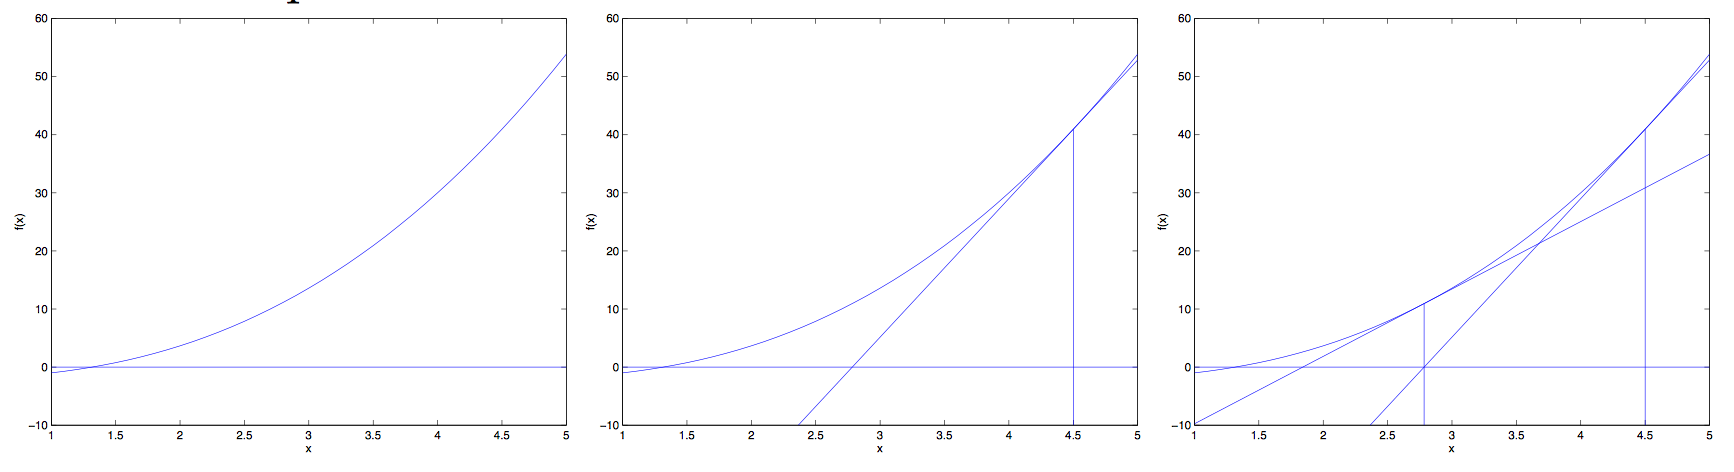
\includegraphics[width=\textwidth]{5.png}
\centering
\end{figure}

在最左边的图里面,可以看到函数 $f$ 就是沿着 $y=0$ 的一条直线。这时候是想要找一个 $\theta$ 来让 $f(\theta)=0$。
这时候发现这个 $\theta$ 值大概在 $1.3$ 左右。加入我们猜测的初始值设定为 $\theta=4.5$。
牛顿法就是在 $\theta=4.5$ 这个位置画一条切线(中间的图)。这样就给出了下一个 $\theta$ 猜测值的位置,
也就是这个切线的零点,大概是 $2.8$。最右面的图中的是再运行一次这个迭代产生的结果,这时候 $\theta$ 大概是 $1.8$。
就这样几次迭代之后,很快就能接近 $\theta=1.3$。

牛顿法的给出的解决思路是让 $f(\theta) = 0$。如果我们要用它来让函数 $\ell$ 取得最大值能不能行呢?
函数 $\ell$ 的最大值的点应该对应着是它的导数 $\ell′(\theta)$ 等于零的点。
所以通过令 $f(\theta) = \ell′(\theta)$,我们就可以同样用牛顿法来找到 $ell$ 的最大值,然后得到下面的更新规则:
\[
	\theta := \theta - \ell'(\theta)/\ell''(\theta).
\]
(额外再思考一下: 如果我们要用牛顿法来求一个函数的最小值而不是最大值,该怎么修改?)

最后,在我们的逻辑回归背景中,$\theta$ 是一个有值的向量,所以我们要对牛顿法进行扩展来适应这个情况。
牛顿法进行扩展到多维情况,也叫\defn{牛顿-拉普森法}{Newton-Raphson method},如下所示:
\[
	\theta := \theta - H^{-1} \nabla_\theta \ell(\theta).
\]
上面这个式子中的 $\nabla_\theta \ell(\theta)$ 和之前的样例中的类似,是关于 $\theta_i$ 的 $\ell(\theta)$ 的偏导数向量;
而 $H$ 是一个 $n \times n$ 矩阵 (实际上如果包含截距项的话,应该是, $(n + 1) \times (n + 1)$),
也叫做\defn{海森矩阵}{Hessian}, 其详细定义是:
\[
	H_{ij} = {\partial^2 \ell(\theta) \over \partial \theta_i \partial \theta_j}.
\]

牛顿法通常都能比(批量)梯度下降法收敛得更快,而且达到最小值所需要的迭代次数也低很多。
然而,牛顿法中的单次迭代往往要比梯度下降法的单步耗费更多的性能开销,因为要查找和转换一个 $n \times n$ 的海森矩阵;
不过只要这个 $n$ 不是太大,牛顿法通常就还是更快一些。当用牛顿法来在逻辑回归中求似然函数 $\ell(\theta)$ 的最大值的时候,
得到这一结果的方法也叫做\defn{费希尔评分}{Fisher scoring}。




\clearpage
\part{广义线性模型\ Generalized Linear Models}

到目前为止,我们看过了回归的案例,也看了一个分类案例。
在回归的案例中,我们得到的函数是 $y|x; \theta \sim \mathcal{N}(\mu, \sigma^2)$;
而分类的案例中,函数是 $y|x; \theta \sim Bernoulli(\phi)$,
这里面的 $\mu$ 和 $\phi$ 分别是 $x$ 和 $\theta$ 的某种函数。
在本节,我们会发现这两种方法都是一个更广泛使用的模型的特例,这种更广泛使用的模型就叫做广义线性模型。
我们还会讲一下广义线性模型中的其他模型是如何推出的,以及如何应用到其他的分类和回归问题上。
\footnote{注:本节内容受以下两份作品的启发:
Michael I. Jordan, \textit{Learning in graphical models} (草稿), 
以及 McCullagh, Nelder, \textit{Generalized Linear Models (2nd ed.)}。
}





\section{指数族\ The Exponential Family}

在学习广义线性模型之前,我们要先定义一下\defn{指数族分布}{exponential family distributions}。
如果一个分布能用下面的方式来写出来,我们就说这类分布属于指数族:
\begin{equation}
	p(y; \eta) = b(y) \exp(\eta^T T(y) - \alpha(\eta)).
\end{equation}

上面的式子中,$\eta$ 叫做此分布的\defn{自然参数}{natural parameter};
$T(y)$ 叫做\defn{充分统计量}{sufficient statistic}(我们目前用的这些分布中通常 $T (y) = y$);
而 $a(\eta)$ 是一个\defn{对数分割函数}{log partition function}。
$e−a(\eta)$ 这个量本质上扮演了\defn{归一化常数}{normalization constant}的角色,
也就是确保 $p(y; \eta)$ 的总和等于 $1$。

对 $T$, $a$ 和 $b$ 的固定选择,就定义了一个用 $eta$ 进行参数化的分布族;
通过改变 $\eta$,我们就能得到这个分布族中的不同分布。

现在我们看到的\defn{伯努利分布}{Bernoulli}和\defn{高斯分布}{Gaussian}就都属于指数分布族。
伯努利分布的均值是 $\phi$,也写作 $Bernoulli(\phi)$,确定的分布是 $y \in \{0, 1\}$,
因此有 $p(y=1; \phi) = phi$ 和 $p(y=0; \phi) = 1-\phi$。
这时候只要修改 $\phi$,就能得到一系列不同均值的伯努利分布了。
现在我们展示的通过修改 $\phi$,而得到的这种伯努利分布,就属于指数分布族;
也就是说,只要给定一组 $T$, $a$ 和 $b$,就可以用上面的等式 $(6)$ 来确定一组特定的伯努利分布了。

我们这样来写伯努利分布:
\begin{align*}
	p(;\phi)
    	&= \phi^y (1-\phi)^{1-y} \\
        &= \exp(y \log \phi + (1-y) \log (1-\phi)) \\
        &= \exp \left\{ \left( \log {\phi \over 1-\phi}\right) y + \log(1-\phi) \right\}.
\end{align*}

因此,自然参数就给出了,即 $\eta = \log (\phi/ (1 − \phi))$。 
很有趣的是,如果我们翻转这个定义,用 $\eta$ 来解 $\phi$ 就会得到 $\phi = 1/ (1 + e^{−\eta} )$。
这正好就是之前我们刚刚见到过的 S 型函数!在我们把逻辑回归作为一种广义线性模型的时候还会遇到这个情况。
为了说明伯努利分布是指数族分布,我们有
\begin{align*}
	T(y) &= y \\
    a(\eta) &= -\log(1-\phi) = \log(1 + e^\eta) \\
    b(y) &= 1
\end{align*}

接下来就看看高斯分布吧。还记得吧,在推导线性回归的时候,$\sigma^2$ 的值对我们最终选择的 $\theta$ 和 $h_\theta(x)$ 都没有影响。
所以我们可以给 $\sigma^2$ 取一个任意值。为了简化推导过程,就令 $\sigma^2=1$\footnote{
如果我们把 $\sigma^2$ 留作一个变量,高斯分布就也可以表达成指数分布的形式,其中 $\eta \in \mathbb{R}^2$ 就是一个二维向量,
同时依赖 $\mu$ 和 $\sigma$。然而,对于广义线性模型方面的用途,$\sigma^2$ 参数就也可以看成是对指数分布族的更泛化的定义:
$p(y; \eta,\tau) = b(a,\tau) exp((\eta^T T(y) − a(\eta))/c(\tau))$。
这里面的 $\tau$ 叫做\defn{分散度参数}{dispersion parameter},
对于高斯分布,$c(\tau) = \sigma^2$;不过上文中我们已经进行了简化,所以针对我们要考虑的各种案例,就不需要再进行更加泛化的定义了。
}。然后就有了下面的等式:
\begin{align*}
	p(;\mu)
		&= {1 \over \sqrt{2 \pi}} \exp\left\{ -{1 \over 2} (y-\mu)^2 \right\} \\
        &= {1 \over \sqrt{2 \pi}} \exp\left\{ -{1 \over 2} y^2 \right\} \cdot 
           \exp\left\{ \mu y - {1 \over 2} \mu^2 \right\}.
\end{align*}
这样,我们就可以看出来高斯分布是属于指数分布族的:
\begin{align*}
	\eta &= \mu \\
	T(y) &= y \\
    a(\eta) &= \mu^2/2 = \eta^2/2 \\
    b(y) &= (1/\sqrt{2\pi}) \exp(-y^2/2).
\end{align*}

指数分布族里面还有很多其他的分布:例如\defn{多项式分布}{multinomial},这个稍后我们会看到;
\defn{泊松分布}{Poisson},用于对计数类数据进行建模,后面再问题集里面也会看到;
\textbf{$\Gamma$分布}和\defn{指数分布}{exponential},这个用于对连续的、非负的随机变量进行建模,例如时间间隔;
\textbf{$\beta$分布}和\defn{狄利克雷分布}{Dirichlet},这个是用于概率的分布;此外还有很多。
在下一节里面,我们就来讲一讲对于建模的一个更通用的“方案”,其中的 $y$(给定 $x$ 和 $\theta$)可以是上面这些分布中的任意一种。






\section{构建广义线性模型\ Constructing GLMs}

设想你要构建一个模型,来估计在给定的某个小时内来到你商店的顾客人数(或者是你的网站的页面访问次数),
基于某些确定的特征 $x$ ,例如商店的促销、最近的广告、天气、今天周几等等。
我们已经知道泊松分布通常能适合用来对访客数目进行建模。知道了这个之后,怎么来建立一个模型来解决我们这个具体问题呢?
非常幸运的是,泊松分布是属于指数分布族的一个分部,所以我们可以使用一个广义线性模型。
在本节,我们讲一种对刚刚这类问题来构建广义线性模型的方法。 

更一般地,设想一个分类或者回归问题,要预测一些随机变量 $y$ 的值,作为 $x$ 的一个函数。
要导出适用于这个问题的广义线性模型,就要对我们的模型给定 $x$ 下 $y$ 的条件分布来做出以下三个假设:
\begin{enumerate}
\item $y|x; \theta \sim ExponentialFamily(\eta)$,即给定 $x$ 和 $\theta$, $y$ 是一个参数为 $\eta$ 的指数分布。
\item 给定 $x$,目的是要预测对应这个给定 $x$ 的 $T(y)$ 的期望值。我们的例子中绝大部分情况都是 $T(y) = y$,
这也就意味着我们的学习假设 $h$ 输出的预测值 $h(x)$ 要满足 $h(x) = \E[y|x]$。 
(注意,这个假设通过对 $h_\theta(x)$ 的选择而满足,在逻辑回归和线性回归中都是如此。
例如在逻辑回归中,$h_\theta(x) = [p(y=1|x;\theta)] = 0 \cdot p (y=0|x;\theta) + 1\cdot p(y = 1|x;\theta) = \E[y|x;\theta]$。)
\item 自然参数 $\eta$ 和输入值 $x$ 是线性相关的,$\eta = \theta^T x$(或者如果 $\eta$ 是向量,则有 $\eta_i = \theta_i^T x$)。
\end{enumerate}

上面的几个假设中,第三个可能看上去证明得最差,所以也更适合把这第三个假设看作是一个我们在设计广义线性模型时候的一种设计选择,
而不是一个假设。那么这三个假设/设计,就可以用来推导出一个非常合适的学习算法类别,也就是广义线性模型,
这个模型有很多特别友好又理想的性质,比如很容易学习。
此外,这类模型对一些关于 $y$ 的分布的不同类型建模来说通常效率都很高;
例如,我们下面就将要简单介绍一些逻辑回归以及普通最小二乘法这两者如何作为广义线性模型来推出。





\subsection{最小二乘法\ Ordinary Least Squares}

我们这一节要讲的是普通最小二乘法实际上是广义线性模型中的一种特例,设想如下的背景设置:
目标变量 $y$(在广义线性模型的术语也叫做\defn{响应变量}{response variable})是连续的,
然后我们将给定 $x$ 的 $y$ 的分布以高斯分布 $\mathcal{N}(\mu, \sigma^2)$ 来建模,
其中 $\mu$ 可以使依赖 $x$ 的一个函数。这样,我们就让上面的指数分布族的 $(\eta)$ 分布成为了一个高斯分布。
在前面内容中我们提到过,在把高斯分布写成指数分布族的分布的时候,有 $\mu = \eta$。所以就能得到下面的等式:
\[
	h_\theta(x) = \E[y|x;\theta] = \mu = \eta = \theta^Tx.
\]
第一行的等式是基于假设 2;第二个等式是基于定理当 $y|x;\theta \sim \mathcal{N}(\mu, \sigma^2)$,
则 $y$ 的期望就是 $\mu$;第三个等式是基于假设 1,以及之前我们此前将高斯分布写成指数族分布的时候推导出来的性质 $\mu = \eta$;
最后一个等式就是基于假设 3。





\subsection{逻辑回归\ Logistic Regression}

接下来我们再来看看逻辑回归。这里我们还是看看二值化分类问题,也就是 $y \in \{0, 1\}$。
给定了 $y$ 是一个二选一的值,那么很自然就选择伯努利分布来对给定 $x$ 的 $y$ 的分布进行建模了。
在我们把伯努利分布写成一种指数族分布的时候,有 $\phi = 1/ (1 + e^{−\eta})$。
另外还要注意的是,如果有 $y|x;\theta \sim Bernoulli(\phi)$,那么 $\E [y|x; \theta] = \phi$。
所以就跟刚刚推导普通最小二乘法的过程类似,有以下等式:
\[
	h_\theta(x) = \E[y|x;\theta] = \phi = 1/(1+e^{-\eta}) = 1/(1+e^{-\theta^Tx}).
\]
所以,上面的等式就给了给了假设函数的形式:$h_\theta(x) = 1/(1+e^{-\theta^Tx})$。
如果你之前好奇我们是怎么想出来逻辑回归的函数为 $1/ (1 + e^{−z})$,这个就是一种解答:
一旦我们假设以 $x$ 为条件的 $y$ 的分布是伯努利分布,那么根据广义线性模型和指数分布族的定义,就会得出这个式子。

再解释一点术语,这里给出分布均值的函数 $g$ 是一个对自然参数的函数,$g(eta) = \E[T(y); \eta]$,
这个函数也叫做\defn{规范响应函数}{canonical response function},
它的反函数 $g^{−1}$ 叫做\defn{规范链接函数}{canonical link function}。
因此,对于高斯分布来说,它的规范响应函数正好就是\defn{识别函数}{identify function};
而对于伯努利分布来说,它的规范响应函数则是逻辑函数。
\footnote{很多教科书用 $g$ 表示链接函数,而用反函数 $g^{−1}$ 来表示响应函数;但是这里用的是反过来的,
这是继承了早期的机器学习中的用法,我们这样使用和后续的其他课程能够更好地衔接起来。}



\subsection{Softmax 回归\ Softmax Regression}

我们再来看一个广义线性模型的例子吧。设想有这样的一个分类问题,其中响应变量 $y$ 的取值可以是 $k$ 个值当中的任意一个,
也就是 $y \in \{1,2,...,k\}$。例如,我们这次要进行的分类就比把邮件分成垃圾邮件和正常邮件两类这种二值化分类要更加复杂一些,
比如可能是要分成三类,例如垃圾邮件、个人邮件、工作相关邮件。这样响应变量依然还是离散的,但取值就不只有两个了。
因此我们就用多项式分布来进行建模。

下面我们就通过这种多项式分布来推出一个广义线性模型。要实现这一目的,首先还是要把多项式分布也用指数族分布来进行描述。

要对一个可能有 $k$ 个不同输出值的多项式进行参数化,就可以用 $k$ 个参数 $\phi_1,...,\phi_k$ 来对应各自输出值的概率。
不过这么多参数可能太多了,形式上也太麻烦,他们也未必都是互相独立的
(比如对于任意一个 $\phi_i$ 中的值来说,只要知道其他的 $k-1$ 个值,就能知道这最后一个了,因为总和等于1)。
所以我们就去掉一个参数,只用 $k-1$ 个,用 $\phi_1,...,\phi_k$ 来对多项式进行参数化,
其中 $\phi_i = p (y = i; \phi)$,$p (y = k; \phi) = 1 − \sum_{i=1}^{k-1}\phi$.
为了表述起来方便,我们还要设 $\phi_k = 1 - \sum_{i=1}^{k-1}\phi$ ,但一定要注意,这个并不是一个参数,
而是完全由其他的 $k-1$ 个参数来确定的。要把一个多项式表达成为指数组分布,还要按照下面的方式定义一个 $T(y)\in\mathbb{R}^{k-1}$:
\[
	T(1) = \begin{bmatrix} 1 \\ 0 \\ 0 \\ \vdots \\ 0 \end{bmatrix},
    T(2) = \begin{bmatrix} 0 \\ 1 \\ 0 \\ \vdots \\ 0 \end{bmatrix},
    T(3) = \begin{bmatrix} 0 \\ 0 \\ 1 \\ \vdots \\ 0 \end{bmatrix},
    \dots,\\
    T(k-1) = \begin{bmatrix} 0 \\ 0 \\ 0 \\ \vdots \\ 1 \end{bmatrix},
    T(k) = \begin{bmatrix} 0 \\ 0 \\ 0 \\ \vdots \\ 0 \end{bmatrix}.
\]
这次和之前的样例都不一样了,就是不再有 $T(y) = y$;此外,$T(y)$ 现在是一个 $k–1$ 维的向量,而不是一个实数了。
向量 $T(y)$ 中的第 $i$ 个元素写成 $(T(y))_i$。

现在介绍一种非常有用的记号。\defn{指示函数}{indicator function} $1\{\cdot\}$,
如果参数为真,则等于 $1$;反之则等于 $0$($1\{True\} = 1$, $1\{False\} = 0$)。
例如$1\{2 = 3\} = 0$, 而$1\{3 = 5 − 2\} = 1$。
所以我们可以把 $T(y)$ 和 $y$ 的关系写成 $(T(y))_i = 1\{y = i\}$。(往下继续阅读之前,一定要确保你理解了这里的表达式为真!)
在此基础上,就有了$\E[(T(y))_i] = P (y = i) = \phi_i$。

现在一切就绪,可以把多项式写成指数族分布了:
\begin{align*}
	p(y;\phi)
    	&= \phi_1^{1\{y=1\}} \phi_2^{1\{y=2\}} \cdots \phi_k^{1\{y=k\}} \\
        &= \phi_1^{1\{y=1\}} \phi_2^{1\{y=2\}} \cdots \phi_k^{1-\sum_{i=1}^{k-1}\{y=i\}} \\
        &= \phi_1^{(T(y))_1} \phi_2^{(T(y))_2} \cdots \phi_k^{1-\sum_{i=1}^{k-1}\{y=i\}} \\
        &= \exp\left\{ (T(y))_1\log(\phi_1) + (T(y))_2\log(\phi_2) 
           + \cdots + \left(1-\sum_{i=1}^{k-1}\{y=i\}\right)\log(\phi_k)\right\} \\
        &= \exp\left\{ (T(y))_1\log(\phi_1/\phi_k) + (T(y))_2\log(\phi_2/\phi_k) 
           + (T(y))_{k-1}\log(\phi_{k-1}/\phi_k) + \log(\phi_k) \right\} \\
        &= b(y) \exp \left\{ \eta^TT(y) - a(\eta) \right\}.
\end{align*}
其中
\begin{align*}
	\eta &= \begin{bmatrix} \log(\phi_1/\phi_k) \\ \log(\phi_2/\phi_k) \\ \vdots \\ \log(\phi_{k-1}/\phi_k) \end{bmatrix} \\
    a(\eta) &= - \log(\phi_k) \\
    b(y) &= 1.
\end{align*}
这样我们就把多项式方程作为一个指数族分布来写了出来。

与 $i$ 对应的链接函数为 $\eta_i = \log(\phi_i / \phi_k)$.
为了方便起见,我们还定义 $\eta_k = \log(\phi_k/\phi_k) = 0$。
对链接函数取反函数然后推导出响应函数,就得到了下面的等式: 
\begin{align}
	e^{\eta_i} &= \phi_i/\phi_k \nonumber \\
    \phi_k e^{\eta_i} &= \phi_i \\
    \phi_k \sum_{i=1}^k e^{\eta_i} &= \sum_{i=1}^k \phi_1 = 1. \nonumber
\end{align}
这就说明了$\phi_k = 1/\sum_{i=1}^k e^{\eta_i}$,然后可以把这个关系代入回到等式上式 $(7)$,这样就得到了响应函数
\[
	\phi_i = {e^{\eta_i} \over \sum_{j=1}^k e^{\eta_j}}.
\]
上面这个函数从 $\eta$ 映射到了 $\phi$,称为 Softmax 函数。

要完成我们的建模,还要用到前文提到的假设 3,也就是 $\eta_i$ 是一个 $x$ 的线性函数。
所以就有了 $\eta_i = \theta_i^Tx (i = 1,...,k-1)$,
其中的 $\theta_1, ..., \theta_{k−1} \in \mathbb{R}^{n+1}$就是我们建模的参数。
为了表述方便,我们这里还是定义 $\theta_k = 0$,这样就有 $\eta_k = \theta_k^Tx = 0$,跟前文提到的相符。
因此,我们的模型假设了给定 $x$ 的 $y$ 的条件分布为:
\begin{equation}
	p(y=i|x;\theta)
    	= \phi_i
        = {e^{\eta_i} \over \sum_{j=1}^k e^{\eta_j}}
        = {e^{\theta_i^Tx} \over \sum_{j=1}^k e^{\theta_j^Tx}}.
\end{equation}
这个适用于解决 $y \in \{1, ..., k\}$ 的分类问题的模型,就叫做 Softmax 回归。 这种回归是对逻辑回归的一种扩展泛化。

我们的假设会输出如下
\[
	h_\theta(x)
    	= \E[T(y)|x;\theta]
        = \E\begin{bmatrix}[c|c] 1\{y=1\} & \\ \vdots & x;\theta \\ 1\{y=k-1\} & \end{bmatrix}
        = \begin{bmatrix} \phi_1 \\ \vdots \\ \phi_{k-1} \end{bmatrix}
        = \begin{bmatrix} {\exp(\theta_1^Tx) \over \sum_{j=1}^k\exp(\theta_j^Tx))} \\ \vdots 
          \\ {\exp(\theta_{k-1}^Tx) \over \sum_{j=1}^k\exp(\theta_j^Tx))} \end{bmatrix}.
\]

也就是说,我们的假设函数会对每一个 $i = 1,...,k$,给出 $p (y = y|x; \theta)$ 概率的估计值。(
虽然咱们在前面假设的这个 $h_\theta(x)$ 只有 $k-1$ 维,但很明显 $p (y = y|x; \theta)$ 
可以通过用 $1$ 减去其他所有项目概率的和来得到)

最后,咱们再来讲一下参数拟合。和我们之前对普通最小二乘线性回归和逻辑回归的原始推导类似,
如果咱们有一个有 $m$ 个训练样本的训练集,$\{(x^{(i)}, y^{(i)}); i = 1, ..., m\}$,
然后要研究这个模型的参数 $\theta_i$,我们可以先写出其似然函数的对数:
\[
	\ell(\theta)
    	= \sum_{i=1}^k \log p(y^{(i)} | x^{(i)}; \theta)
        = \sum_{i=1}^k \log \prod_{l=1}^k 
          \left( {e^{\theta_l^Tx^{(i)}} \over \sum_{j=1}^k e^{\theta_j^Tx^{(i)}}}\right)^{1\{y^{(i)} = l\}}.
\]
要得到上面等式的第二行,要用到等式 $(8)$ 中的设定 $p(y|x; \theta)$。
现在就可以通过对 $\ell(\theta)$ 取最大值得到的 $\theta$ 而得到对参数的最大似然估计,使用的方法就可以用梯度上升法或者牛顿法了。



\end{document}














